\documentclass[12pt, a4paper]{article}
\usepackage[latin2]{inputenc}
\usepackage{graphicx}
\usepackage{ulem}
\begin{document}






\begin{center}\end{center}

\begin{center}\end{center}

\begin{center}\end{center}

\begin{center}\end{center}

\begin{center}\end{center}

\begin{center}\end{center}



\begin{center}\end{center}

\begin{center}\textbf{A New Concept of Effective Regression Test 
}\end{center}

\begin{center}\textbf{Generation in a C++ Specific Environment}
\end{center}











\begin{center}Mih�ly Bicz�$^{1}$, Kriszti�n P�cza$^{1}$, Istv�n 
Forg�cs$^{2}$, Zolt�n Porkol�b$^{1}$\end{center}



$^{1}$E�tv�s Lor�nd University, Fac. of Informatics, Dept. of Prog. 
Languages and Compilers,\\
P�zm�ny P�ter s�t�ny 1/c. H-1117, Budapest, Hungary

mihaly.biczo@axelero.hu, kpocza@kpocza.net, gsd@elte.hu



$^{2}$4D SOFT Ltd. Telepy u. 24. H-1212, Budapest, Hungary

forgacs@4dsoft.hu

\begin{center}\end{center}

\begin{center}\end{center}

\begin{center}\end{center}

\textbf{Abstract}



During regression testing test cases from an existing test suite are run 
against a modified version of a program in order to assure that the 
underlying modifications do not cause any side effects that would 
demolish the integrity and consistency of the system. Since the ultimate 
goal of a regression test set is to effectively test all modifications 
and reveal errors in the earliest possible stage, the maintenance of a 
relevant test set containing effective test cases is of utmost 
importance. In this paper we present an efficient, C++ specific 
framework to automatically manage the regression test suite. Our two 
main contributions are a new interpretation of reliable test cases and a 
dynamic forward impact analyzer method that eases the transformation 
of existing tests to meet the definition of reliability. Using this 
approach we complement the test set with test cases that pass through a 
modification and have an impact on at least one output. Our approach is 
designed to be applicable to large-scale applications. 



\textbf{\textit{Keywords}}: regression testing, dynamic impact 
analysis, software maintenance, C++



\section{\newpage
\textbf{1 Introduction}}


Regression testing is an important tool of software engineers to 
successfully manage issues rising during the evolution of large software 
systems. During the lifetime of large systems numerous modifications are 
performed over possibly many years, yet it is of vital importance that 
none of these modifications is allowed to remain untested, or cause 
unwanted and undiscovered side effects to other previously tested parts.

In order to achieve this goal, a regression test set that covers the 
whole system has to be maintained and adjusted according to the 
modifications performed. Therefore, it is desirable to find a test 
selection method that selects those and only those test cases that might 
reveal an error $[$7$]$. However, it is equally important to re-use 
and transform existing test cases so that the coverage of the modified 
system would not be affected. 

An important subset of regression tests contains \textit{modification 
revealing tests} for which the original and modified programs give 
different output. All modification revealing tests are \textit{
modification traversing}, they necessarily reach at least one modified 
statement. Consequently, the set of modification traversing tests also 
contains all error revealing test cases $[$17$]$. Unfortunately, the 
reverse case is not true: a modification traversing test is not 
necessarily modification revealing. Existing methods consider a test 
case successful if the outputs of the original and modified programs are 
identical. As it can be seen easily, using this approach it is not 
assured that the modification is really tested. In other words, the test 
case is not necessarily reliable.

In this paper we alter the existing definition of reliability: the 
definition of a reliable test pair will be established. According to 
this definition, we develop an approach that eases the generation of 
reliable test pairs in a C++ specific environment. We will not cover 
test data generation techniques, related work can be found in $[$2, 3, 
10, 11$]$. Instead, we identify those input variables from the whole 
state space on which the new generation process can be started. For the 
generation process, the method described in $[$18$]$ can be used 
initiated on a reduced input variable set. 

Our main contribution is a simple forward dynamic impact analyzer 
algorithm which, if there is a given modification, will efficiently 
select the set of influencing input variables and help boost the 
performance of the test pair generation process. As opposed to existing 
methods $[$15$]$, instead of directly comparing the output of the 
original and modified programs for a given test case, the modified 
program and the underlying test case are considered. The test suite will 
be extended with a reliable test pair that is derived from the 
original test. This test pair will assure that the modification is 
tested and that some output statements are affected. An additional 
benefit of our approach is that it is designed to work for real C++ 
based systems, since many C++ specific constructs are covered including 
pointers and function pointers as well as object-oriented constructs and 
paradigms like classes, inheritance and polymorphism.

The structure of the paper is the following: Section 2 defines the 
problem we are going to solve and presents the general overview of the 
generator framework through simple examples. 

In Section 3 we discuss some related work and research directions we are 
aware of. We will primarily focus on the motivating ideas behind 
existing techniques. 

In Section 4 an overview of the used notations and necessary language 
specific instrumentation mechanism will be described in detail.

In Section 5 and Section 6 the two stages of the dynamic forward input 
analyzer algorithm that detects affecting input variables will be 
discussed. While the first stage of the algorithm categorizes test case
s and identifies affected statements; the second stage selects the 
underlying input variables based on the results of the first phase. 

In Section 7 a full example of our approach will be presented in C++.

In Section 8 we summarize our results and discuss the limitations of the 
approach as well as some possible research directions.



\section{\textbf{2 Framework overview}}


\subsection{2.1 The necessity of a concept change}


As we have mentioned in the introductory section, traditional regression 
testing approaches categorize test cases based on the outcome of the 
test case run against the original and the modified programs. However, 
many anomalies might prevent this comparison from being a good filter 
of errors.

The fundamental issue is that if a modification traversing test gives 
identical output for the original and modified programs, this does not 
mean that any of the modifications have really been tested. This is the 
case when a given modification does not affect any output statements. 
The reverse case - when the outcome of the original and modified progra
ms differs - can also be problematic, because the test might not be 
modification traversing for a given modification. As a consequence if 
there are more than one modifications (which is typically the case), 
classical modification revealing tests might not be effective, and once 
again untested modifications might lurk in the source code. A further 
example for different output is when the mistakenly modified statement 
is a predicate, and the test takes another execution branch, although it 
should go along the original path.

int main()

\{

\ \ \ \ double a,b,c, d;



\ \ \ \ cin $>$$>$ a;

\ \ \ \ b=3; //Modification \#1: b=2;

\ \ \ \ c=3;



\ \ \ \ d=a+c;



\ \ \ \ if(a$>$0)

\ \ \ \ \ \ \ \ cout $<$$<$ b $<$$<$ endl;

\ \ \ \ else

\ \ \ \ \ \ \ \ cout $<$$<$ c+2 $<$$<$ endl; //Modification \#2



\ \ \ \ //Use d...



\ \ \ \ exit(0);

\}

int main()

\{

\ \ \ \ double a,b,c, d;



\ \ \ \ cin $>$$>$ a;

\ \ \ \ b=2;

\ \ \ \ c=3;



\ \ \ \ d=a+c;



\ \ \ \ if(a$>$0)

\ \ \ \ \ \ \ \ cout $<$$<$ b $<$$<$ endl;

\ \ \ \ else

\ \ \ \ \ \ \ \ cout $<$$<$ c $<$$<$ endl;



\ \ \ \ //Use d...



\ \ \ \ exit(0);

\}

int main()

\{

\ \ \ \ double a,b,c, d;



\ \ \ \ cin $>$$>$ a;

\ \ \ \ b=2;

\ \ \ \ c=3;



\ \ \ \ d=a-c; //Modification \#1: d=a+c;



\ \ \ \ if(a$>$0)

\ \ \ \ \ \ \ \ cout $<$$<$ b $<$$<$ endl;

\ \ \ \ else

\ \ \ \ \ \ \ \ cout $<$$<$ c $<$$<$ endl;



\ \ \ \ //Use d...



\ \ \ \ exit(0);

\}



\begin{center}Listing 1. \textbf{Three versions of a simple program }
\end{center}



Let's consider the three different versions of a simple program in L
isting 1. If the input of the program (the test case) is a=1, then the 
outcome of the original program is that 2 is printed on the screen. The 
second version still prints 2 for a=1, which is a modification 
traversing test case, and it is successful even though no modifications 
have been tested. In the third version there are two modifications. 
Although for a=1 the outcome of the original and modified programs 
differs, the test case is still not modification traversing for 
Modification \#2. Although these simple examples show only two possible 
anomalies, theoretically, there are four of them: If the test case does 
not traverse any modifications, the output cannot be affected (S0). The 
other three types of the same output symptom are \textit{coincidental 
correctness} (S1); \textit{predicate-only symptom}, e.g. the 
modification influences (either directly or indirectly) only a predicate 
(S2); or the \textit{modified statement does not affect any output} 
(S3).



\subsection{2.2 The changed concept}


In order to overcome the above mentioned shortcomings, we have to 
introduce a new regression testing concept and criterion. Our goal is 
to test each modification in such a way that - if possible - after the 
test traverses the location of the modification at least one output 
statement would be affected. Of course the original test suite might not 
contain tests that meet this criterion, so it is desirable to establish 
a method that transforms all possibly usable regression test cases. 
This way, errors can be revealed with a much higher probability and in 
an earlier stage.



Naturally, to detect a faulty modification, the underlying test case 
has to 

\newcounter{numberedCntL}
\begin{enumerate}
\item reach the fault (it has to be modification traversing with respect 
to the faulty modification) 
\item the inner state of the program has to be erroneous (the behavior 
of the program has to differ from the expected)
\item the fault has to reach an output statement resulting in a failure 
(after the traversal through the erroneous statement, an output 
statement should be reached)
\setcounter{numberedCntL}{\theenumi}
\end{enumerate}


Common methods consider a test case successful if the outputs of the 
original and modified programs are identical. The biggest concept change 
is that we fulfill these requirements using a pair of test cases derived 
from the original test case instead of just one test. 



\subsection{2.3 The test generator framework}


We build our framework around the above set of criteria. We have had a 
strong cooperation with an industrial partner, and the framework we 
present in this paper is part of their project. 

In order to fulfill the first requirement, modification traversing test 
cases have to be selected for a given (possibly erroneous) 
modification. Different techniques can be found in $[$6, 8, 9$]$. 
Identifying modification traversing test cases requires two steps:

\newcounter{numberedCntW}
\begin{enumerate}
\item The modification needs to be detected
\item Appropriate test cases have to be identified
\setcounter{numberedCntW}{\theenumi}
\end{enumerate}
Of course in the case of real software systems extending possibly 
millions of lines of code, it is far from being trivial to identify 
each modification in source code. Our industrial partner has a static 
analyzer solution that identifies modifications within due time for 
millions of lines of code. Although the algorithm and the 
implementation is part of a commercial application, for publicly 
accessible implementation the Columbus framework $[$12$]$ could be used.



In order to fulfill the second requirement, we establish the following 
definition of reliable test cases:



\textbf{Definition (Reliable test pair).} Let GI=\{I$_{1}$, I
$_{2}$, ... I$_{M}$\} the set of input variables, I
\begin{figure}[h]
\centering

\includegraphics[width=12.25pt,height=12.25pt]{media/image1.eps}
\end{figure}
\{1,...M\}, I=\{i$_{1}$,i$_{2}$,...i$_{n}$\}, J
\begin{figure}[h]
\centering

\includegraphics[width=12.25pt,height=12.25pt]{media/image1.eps}
\end{figure}
\{1,...M\}, J=\{j$_{1}$,...j$_{k}$\} index sets. Consider the 
following test cases: t$_{1}$:=$<$i$_{i1}$, i$_{i2}$, ... i
$_{in}$$>$, t$_{2}$:=$<$i$_{j1}$,i$_{j2}$,...i$_{jk
}$$>$, where i$_{i1}$, i$_{i2}$,... i$_{in}$, i$_{j1}$, 
i$_{j2}$, ... i$_{jk}$ are the values of the corresponding input 
variables. A pair (t$_{1}$, t$_{2}$) of test cases is a 
reliable test pair with respect to statement s$^{q}$ (where s$^{q
}$ represents the q$^{th}$ execution of statement s) if t$_{1}$ 
and t$_{2}$ travels along the same execution path until s$^{q}$, 
the result of s$^{q}$ differs for t$_{1}$ and t$_{2}$, and t
$_{1}$ and t$_{2}$ are 'close' to each other (for numeric values 
the difference should be minimized according to some metric).



Informally, the above definition says that a test case is reliable with 
respect to a given modification if and only if the two test cases 
generate the same execution path as far as s$^{q}$, both of them ha
ve an influence on at least one output statement, and the result of the 
output statements differ for the two test cases. Besides this, their 
difference should be minimized according to the following rule: the 
number of common variables in set I and J should be minimized, and for 
the common variables, the difference between them should be minimized 
according to some metric. For the Eucledian metric, this would be



\begin{center}\begin{figure}[h]
\centering
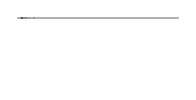
\includegraphics[width=78.15pt,height=31.65pt]{media/image2.eps}
\end{figure}
\end{center}



As for the third requirement, we will assume that all test cases in 
this case reach a modification. Some of them will have an influence on 
the output, some of them will not. However, in both cases it is highly 
desirable to transform them to a test pair that meets the definition of 
reliability. 

For the effective generation of test cases that meet the definition of 
our regression testing criterion, we need a reduced set of input 
variables. This is the main task we solve in this paper: according to 
the altered definition of reliable test cases (reliable test pair), we 
are to reduce the set of input variables to so-called influencing input 
variables. These are input variables that can be used to generate 
reliable test pairs based on a modification traversing test case. 

Our suggested solution for finding influencing input variables is a two 
stage process. In the first stage the symptom (the anomaly that the test 
case causes, S0-S3) is determined. In the second phase the set of 
influencing input variables are identified which can be used to turn the 
underlying test case to a reliable test pair. Both stages of the 
algorithm are based on \textit{forward dynamic impact analysis}. 
Consequently, there is no need for large data structures in memory, and 
all results can be obtained on-the-fly. The high-level structure of the 
framework is the following:



\newcounter{numberedCntX}
\begin{enumerate}
\item Identify modifications
\item Select modification traversing test cases from the original test 
suite
\item For each selected test case
\begin{enumerate}
\item Identify symptom (S1, S2, S3)
\item Identify reduced set of influencing input variables
\end{enumerate}
\item Generate a test pair in the reduced variable space using 
influencing input variables
\setcounter{numberedCntX}{\theenumi}
\end{enumerate}


Our main contributions are 3a and 3b. The schematic structure can be 
seen in the following figure (Our contributions are in the dark 
rectangle).





\section{\textbf{3 Related work, research directions}}


In this section we present related work that motivated our research. 
$[$19$]$ deals with the empirical comparison of test selection 
techniques. Besides the commonly used but rather desperate random and 
retest all techniques, minimization, dataflow and safe test selection 
families are also covered in that paper. Our suggested approach has 
common properties with dataflow techniques that require that every 
definition-use pair that is deleted, changed, or inserted into the 
program to be tested. In $[$20$]$ Harrold and Sofa select test cases 
that exercise the definition-use pairs affected by the modification. Our 
approach is quite similar with the important difference that we employ 
test pairs that are safer in case of predicates and require not only the 
testing of the modification, but also the employment of at least one 
output statement.

The two most relevant papers that motivated our research are $[$16$]$ 
and $[$17$]$. The first paper deals with slicing $[$5$]$ algorithms 
that do not use traditional data structures, only dependence analysis to 
calculate program slices. The second paper categorizes regression test 
cases based on their effect on the program output. We try to compose and 
further simplify these approaches to reduce the set of input variables 
on which new reliable regression test case generation can be based.



\subsection{3.1 Graph-less dynamic slicing and impact analysis}


In $[$16$]$ a new approach to producing dynamic program slices is 
proposed. The main idea of the work is to employ dependence analysis 
to dynamic slicing $[$1, 13, 14$]$ instead of applying traditional 
techniques that usually require a graph-based representation and might 
seriously confine application possibilities due to memory consumption. 
The dynamic dependences that are tracked are the same as in the case 
of the graph representation, but instead of one huge graph, various data 
structures are maintained.

Besides introducing alternative dependence-based methods, slicing 
scenarios are categorized $[$5$]$ based on slicing direction, 
processing direction and global or demand-driven nature of the 
algorithm. Our impact analysis that will be presented in Section 5 
relate closely to the forward, demand driven algorithm in $[$16$]$. The 
difference between the two approaches lies in the fact that we will not 
produce dynamic slices; therefore different data structures will be 
maintained. The reason why we do not apply dynamic slicing is that we 
need only a set of variables, and not a slice of the entire program.

 

\subsection{3.2 Mutation-based regression testing}


Paper $[$17$]$ deals with regression test generation. The generation 
process has two stages: in the first stage existing test cases are 
categorized similarly to the previously mentioned (S0, S1, S2, S3) 
cases. Based on the outcome of the first stage, a new test case will be 
generated that effectively tests a modification. Our work is derived 
from that article; however, there are a few important improvements. 
First of all, we allow more than one modification to occur in the 
source code, and generate not only a test case, but a test pair. The 
test pair should match the changed definition of reliability.



\section{\textbf{4 Tools and notations}}




In order to perform dynamic impact analysis, the source code has to be 
carefully instrumented. During the execution of the instrumented code 
each traversal through a previously inserted sensor is registered. We 
will show that it is not necessary to maintain a log file (which again 
can grow huge) and log the registered traversal. 

The relatively complex instrumentation that is required for real C++ 
code can be performed using various tools, like the Columbus framework 
$[$12$]$. In the following we briefly describe the used notations and 
the information that instrumentation must provide. We are going to 
employ sequence-point level instrumentation, which means that sensors 
are inserted after each sequence point. This might imply that the trace 
can grow too large to handle, however, as we will see, it can be 
produced and processed on the fly.

For the identification of types, their fully qualified name is used (
namespace1::namespace2::...::Class1::Class2..)

All typedefs have to be resolved so that their corresponding type that 
can be identified.

For the unique identification of variables, we use the following 
notation:



D(v, s, q, A$_{v}$, A$_{p}$),



where v is the fully qualified name of the variable, s is the 
identification number of the statement which runs the q$^{th}$ time, 
and v appears in the q$^{th}$ run of s. Since C++ support pointer 
types, we have to distinguish between the memory location where the 
variable resides, and the memory location it points to in case it is a 
pointer. A$_{v}$ represents the memory location of the variable, and 
A$_{p}$ is the pointed memory location (for non-pointer typed 
variables, A$_{v}$ and A$_{p}$ are equivalent). A variable can 
be either global, static, local, or member variable. For the latter



DD(D$_{object}$, D$_{member}$) 



notation is used. Let's consider the example when there is a class named 
Foo and there is a Bar typed member variable in it with the name b. When 
we instantiate an object of Foo at a uniquely identified program 
location, both members of the DD pair can be filled in.



(s, q): Foo f;



And we would like to describe the member b. Then the following entry 
will be generated:



DD(D(Foo::f, s, q, 0x13217ffa4, 0x13217ffa4), 

 D(Bar::b, s, q, 0x1322a4c28, 0x1322a4c28))



Static, local or global variables can also be described this way with D
$_{object}$ being NULL in these cases.

For local variables the fully qualified name has to be integrated with 
the exact block number where the local variable is defined. Pointer and 
function pointer variables can be described similarly. 

At each sequence point along the execution path we have to record the 
defined (DEF) and used (USE) variables, and each variable has to be 
identified with the above specified granularity. (Both of them contain 
variables that are identified using the DD notation above.)

At each function we store the exact signature along with the source 
code location in the call stack.

C++ rigorously defines destructors to be run deterministically when 
execution leaves scope, or when an explicit delete is requested. 
Destructors should be instrumented just like ordinary functions, but 
with virtual or estimated line or column number.

Another instrumentation requirement is in connection with the lazy 
evaluation strategy of C++. Only those variables should appear in the 
instrumentation log that are really used or defined. In the following we 
will refer to these variables as actually defined/actually used 
variables.



\section{\textbf{5 Forward symptom analyzer algorithm}}


In this section we present our forward dynamic impact analysis 
algorithm. 

As we have shown previously, it is possible to identify memory locations 
for each variable. Consequently, it is not necessary to start our 
algorithm from the beginning of the program, rather from the location of 
the first occurrence of the modified statement. However, this approach 
implicitly implies that the execution history of the test case is the 
same for the original and modified programs until the first occurrence 
of the modification. Unfortunately, the execution history can be too 
large to log and to keep in memory, and the solution would not have a 
significant advantage over dynamic slicing.

To overcome this difficulty, it is also possible to start the algorithm 
from the very beginning of the program, and employ an online algorithm 
that processes log entries on-the-fly. By online we mean that the 
instrumentation sensors write the log entries to a buffered stream, and 
the impact analyzer fetches them on-the-fly. Although this way a slight 
performance loss occurs, but we gain significant advantage in the field 
of storage and memory consumption, which are usually the critical 
factors. 

Therefore, the input of the algorithm is not the execution history, 
rather a test case that has previously been selected. The algorithm will 
identify both the same-output symptom (S1/S2/S3) and the affected output 
statement or predicate (P).

Along the execution path, all variables have to be meticulously 
identified and tracked in order to easily maintain the DEF and USE sets 
at each sequence point. To achieve this goal, all kinds of assignment 
operations between variables need to be described in terms of the above 
notations. Originally, we treated simple (built-in) and user-defined 
types separately, but it turned out that it is not necessary to make 
distinction between the two categories. Since these two elements take 
the same form, we explain only the assignment of simple (local) 
variables. Different cases are shown in . In the first column the 
possible types of underlying variables and the location of their 
definition is shown. The second column contains the assignment 
operations again with the location, while in the third column the 
instrumentation entry can be seen. The format of the entry takes the 
following form: L stands for assignment location, R for actually 
referenced variable, D for defined variable. Please note that the 
location means a sequence point.



\begin{table}[h]
\centering
\begin{tabular}{|l|l|l|}
\hline
\textbf{Variable types and locations} & \textbf{Assignment loca
tion/ operation} & \textbf{Instrumentation entry} \\
\hline
(Si,Qi) int i;(Sj,Qj) int j;  & (S,Q) i= j; & \textit{L: (S,Q)R: D(j, 
Sj, Qj, Avj, Avj)D: D(i, Si, Qi, Avi, Avi)} \\
\hline
(Si,Qi) int *i; (Sj,Qj) int *j; & (S,Q): i = j; & \textit{L: (S,Q)R: 
D(j, Sj, Qj, Avj, Apj)D: D(i, Si, Qi, Avi, Apj)} \\
\hline
(Si,Qi) int *i; (Sj,Qj) int j; & (S,Q): i = \&j; & \textit{L: (S,Q)R: 
D(j, Sj, Qj, Avj, Avj)D: D(i, Si, Qi, Avi, Avj)} \\
\hline
(Si,Qi) int *i; (Sj,Qj) *j;int a; & (S,Q): i = j+2+a; & \textit{L: 
(S,Q)R: D(j, Sj, Qj, Avj, Apj)D: D(i, Si, Qi, Avi, 
Apj+sizeof(*j)*(2+a))} \\
\hline
(Si,Qi) int *i;(Sj,Qj) int *j; & (S,Q): *i = *j; & \textit{L: (S,Q)
R: D(j, Sj, Qj, Avj, Apj)D: D(i, Si, Qi, Avi, Api)} \\
\hline
(Si,Qi) int *i;(Sj,Qj) int j; & (S,Q): *i = j; & \textit{L: (S,Q)R: 
D(j, Sj, Qj, Avj, Avj)D: D(i, Si, Qi, Avi, Api)} \\
\hline
(Si,Qi) int *i;  & (S, Q): i = new int; & \textit{L: (S,Q)R: -D: D(i, 
Si, Qi, Avi, ApiNew)} \\
\hline
\end{tabular}
\caption{\label{table:_Ref131150015}: Assignment of primitive types}
\end{table}



As we have previously mentioned, the assignment of primitive types can 
be applied to user-defined types as well, although there are some 
important extensions. C++ allows programmers to overload default 
operators, including the assignment operator. If there is no explicit 
user defined assignment operator in a class, then the default assignment 
operator (member-wise assignment) is applied. On the other hand, if 
there is a custom assignment operator, its effect has to be preserved in 
the execution history.

At this point we have all the necessary information to describe the 
intra-procedural version of the forward dynamic symptom analyzer 
algorithm. Later, it will be extended to its final inter-procedural 
form.

The input of the algorithm is the test case, the location of the 
modification, and the set of variables that are defined at the modified 
statement. Because the set of defined variables at the modification is 
not known, and generating the whole execution trace is not acceptable, 
the values of the actually defined variables have to be calculated in a 
preprocessing step. 

int n = 2;

int *ip = *jp = \&n;

//modification:

*ip = 3; //original: *ip = 6;

...

if(*jp $>$ 5)

Listing 2\textbf{: Pointer example}

The preprocessing step requires the introduction of a set that stores 
variables of interest along the execution path. This set will be 
referred to as \textit{Varstore}. \textit{Varstore} is set to empty
. At each variable assignment the defined variable calculated based on 
rules listed in  is added to \textit{Varstore}. When execution leave
s the scope, all local variables will be removed. The same case holds 
when an explicit delete operation is requested. When we reach the first 
occurrence of the modified statement, the memory location of the 
actually defined variables can be calculated, and the set \textit{
Varstore} can be deleted. The introduction of \textit{Varstore} is 
important because of the pointer typed variables of C++. Consider the 
example in Listing 2. All three variables (\textit{n}, \textit{ip
}, \textit{jp}) will be added to \textit{Varstore}, and at the 
predicate we can detect that we refer to the same variable that was 
modified.



After the initialization step we introduce a set called \textit{Affect
} for storing variables that are directly or indirectly affected by 
variables defined at the modified statement. The main steps of our 
algorithm without the preprocessing step are the following. 



\newcounter{numberedCntB}
\begin{enumerate}
\item \textit{Affect }is initialized with variables that are defined 
at the modified statement i$_{mod}$\textit{ }and refer to the same 
memory location\textit{ }(based on \textit{Varstore}), starting 
point is set to i$_{mod}$.
\item From i$_{mod}$\textit{ } we traverse over statements (i$_{q
}$) along the execution path according to test case T, and based on 
the type of this statement, we take one of the following actions:
\begin{enumerate}
\item If i$_{q}$ is an output statement (in other words it is not a 
predicate and does not define variables), and there is at least one used 
variable from \textit{Affect}, then the underlying symptom is 
trivially S1, and the affected statement is sq, in addition the 
algorithm can safely terminate.
\item If i$_{q}$ is a predicate, then all actually used variables are 
considered. If the intersection of this set and \textit{Affect} is not 
empty, then S2 is identified, and the affected statement is i$_{q}$. 
When predicate i$_{q }$is the modified statement then S2 is also 
identified at the modified statement.
\item If i$_{q}$ is an assignment, then for each w variable used at i
$_{q}$ the presence of the variable in \textit{Affect} is checked. 
If a w variable is in \textit{Affect} then the defined variables in i
$_{q}$ are added to \textit{Affect}. The statement defining w is 
marked as effective.\\
For each w variable in \textit{Affect} it is checked if the w 
variable is defined at i$_{q}$ and the last definition of w is not at 
i$_{q. }$If the previous condition is true then w is removed from 
\textit{Affect}, moreover if the last definition is not effective 
the S3 is identified.
\setcounter{numberedCntB}{\theenumi}
\end{enumerate}
\end{enumerate}


In order to successfully extend this algorithm to the inter-procedural 
case, we have to address parameter passing methods, and return values as 
well.



\begin{table}[h]
\centering
\begin{tabular}{|l|l|}
\hline
\textbf{Method} & \textbf{Modelling} \\
\hline
By valueThe same as (int i=j) & \textit{D(j, Sj, Qj, Avj, Avj)D(i, 
Si, Qi, Avi, Avi)} \\
\hline
By addressThe same as (int*i=\&j) OR(int *i=j) if j is a pointer & 
\textit{D(j, Sj, Qj, Avj, Avj)D(i, Si, Qi, Avi, Avj)}OR\textit{
D(j, Sj, Qj, Avj, Apj)D(i, Si, Qi, Avi, Api)} \\
\hline
By reference & \textit{D(j, Sj, Qj, Avj, Avj)D(i, Si, Qi, Avj, Avj)} 
\\
\hline
\end{tabular}
\caption{\label{table:_Ref131150951}: Parameter passing methods and 
their representation}
\end{table}

Function FindInfluencingInputs(T, V)

Affect=\{\}

for each statement i$_{q}$ in ExecutionPath(T) from i$_{first}$ to 
i$_{last }$do

begin

\ \ \ \ if i$_{q}$ is input statment then

\ \ \ \ begin

\ \ \ \ \ \ \ \ Affect=Affect U i$_{q}$.Def $_{(iq.Def)}$

\ \ \ \ end

\ \ \ \ if i$_{q}$ is predicate then

\ \ \ \ begin

\ \ \ \ \ \ \ \ for each u in i$_{q}$.ExecConditions.Use do

\ \ \ \ \ \ \ \ begin

\ \ \ \ \ \ \ \ \ \ \ \ if u$_{(v)}$  Affect then

\ \ \ \ \ \ \ \ \ \ \ \ begin

\ \ \ \ \ \ \ \ \ \ \ \ \ \ \ \ V(i$_{q}$)=V(i$_{q}$) U v

\ \ \ \ \ \ \ \ \ \ \ \ end

\ \ \ \ \ \ \ \ end

\ \ \ \ end

\ \ \ \ if i$_{q}$ is definition or function return then

\ \ \ \ begin

\ \ \ \ \ \ \ \ for each d  i$_{q}$.Def do

\ \ \ \ \ \ \ \ begin

\ \ \ \ \ \ \ \ \ \ \ \ for each d$_{(v)}$  Affect do

\ \ \ \ \ \ \ \ \ \ \ \ begin

Affect=Affect $\backslash$ d$_{(v)}$

\ \ \ \ \ \ \ \ \ \ \ \ end

\ \ \ \ \ \ \ \ end

\ \ \ \ \ \ \ \ for each j  i$_{q}$.Use ? Affect.Indices do

\ \ \ \ \ \ \ \ begin

\ \ \ \ \ \ \ \ \ \ \ \ Affect=Affect  \{i$_{q}$.Def$_{(j)}$\}

\ \ \ \ \ \ \ \ end

\ \ \ \ \ \ \ \ for each w  i$_{q}$.Use do

\ \ \ \ \ \ \ \ begin

\ \ \ \ \ \ \ \ \ \ \ \ for each w$_{(j)}$  Affect 

\ \ \ \ \ \ \ \ \ \ \ \ begin

\ \ \ \ \ \ \ \ \ \ \ \ \ \ \ \ Affect=Affect  \{i$_{q}$.Def$_{(j)
}$\}

\ \ \ \ \ \ \ \ \ \ \ \ end

\ \ \ \ \ \ \ \ end

\ \ \ \ end

\ \ \ \ if i$_{q}$ is function call then

\ \ \ \ begin

\ \ \ \ \ \ \ \ AssignParams(i$_{q}$)\ \ \ \ 

end

end

Listing 4\textbf{: Influencing inputs}

Function SymptomAndLocation(T, S, P)

Affect=\{i$_{mod}$.Def\}

S = Nothing

for each statement i$_{q}$ in ExecutionPath(T) from i$_{mod}$ to i
$_{last }$do

begin

\ \ \ \ if i$_{q}$ is output and i$_{q}$.Use?Affect   then

\ \ \ \ begin

\ \ \ \ \ \ \ \ S = S1;

\ \ \ \ \ \ \ \ P = i$_{q}$;

\ \ \ \ \ \ \ \ terminate;

\ \ \ \ end

\ \ \ \ if i$_{q}$ is predicate and (i$_{q}$.Use?Affect  \\
 or i$_{q}$ is the modified statement) then

\ \ \ \ begin

\ \ \ \ \ \ \ \ S = S2;

\ \ \ \ \ \ \ \ P = i$_{q}$;

\ \ \ \ \ \ \ \ terminate;

\ \ \ \ end

\ \ \ \ if i$_{q}$ is definition or function return then

\ \ \ \ begin

\ \ \ \ \ \ \ \ for each w  i$_{q}$.Use do

\ \ \ \ \ \ \ \ begin

\ \ \ \ \ \ \ \ \ \ \ \ if w  Affect then

\ \ \ \ \ \ \ \ \ \ \ \ begin

\ \ \ \ \ \ \ \ \ \ \ \ \ \ \ \ Affect=Affect U i$_{q}$.Def

\ \ \ \ \ \ \ \ \ \ \ \ \ \ \ \ mark d$^{w}$ as effective

\ \ \ \ \ \ \ \ \ \ \ \ end

\ \ \ \ \ \ \ \ end

\ \ \ \ \ \ \ \ for each w  Affect do

\ \ \ \ \ \ \ \ begin

\ \ \ \ \ \ \ \ \ \ \ \ if w ? i$_{q}$.Def and d$^{w}$$<$$>$ i
$_{q}$ then

\ \ \ \ \ \ \ \ \ \ \ \ begin

\ \ \ \ \ \ \ \ \ \ \ \ \ \ \ \ Affect=Affect$\backslash$\{w\}

\ \ \ \ \ \ \ \ \ \ \ \ \ \ \ \ if d$^{w}$ is not effective then

\ \ \ \ \ \ \ \ \ \ \ \ \ \ \ \ begin

\ \ \ \ \ \ \ \ \ \ \ \ \ \ \ \ \ \ \ \ S=S3

\ \ \ \ \ \ \ \ \ \ \ \ \ \ \ \ \ \ \ \ P=i$_{q}$

\ \ \ \ \ \ \ \ \ \ \ \ \ \ \ \ end

\ \ \ \ \ \ \ \ \ \ \ \ end

\ \ \ \ \ \ \ \ end

\ \ \ \ end

\ \ \ \ if i$_{q}$ is function call then

\ \ \ \ begin

\ \ \ \ \ \ \ \ AssignParams(i$_{q}$)\ \ \ \ 

end

end

Listing 3\textbf{:} \textbf{Symptom analyzer}





In C++ parameters can be passed via one of the following methods: by 
value, by address, and by reference. 

Within a function any assignment to a parameter that has previously been 
passed by reference will not take effect outside the function, yet these 
assignments can alter the execution path through the return value of the 
function. A parameter passing by value can be modeled as an assignment 
to a local variable.

Parameter passing by address means the passing of pointer variables. Any 
assignment to a pointer variable within a function will not cause any 
side effect outside. Nevertheless, with the modification of the pointed 
memory location via dereference (*) operator side effects may occur. 
Passing by address can be thought of as introducing a new local pointer 
variable originally set to the same memory location as the pointed 
memory location of the actual parameter.

Since a reference can be regarded as the synonym of a memory location, 
any modification to a parameter passed by reference will take effect 
outside the function.

The three cases are summarized in  using the previously introduced 
notation. Please note that j represents the actual parameter, while i 
is the formal parameter.

In order to complete our extension, we have to cover the handling of 
return values. The return statement can also be substituted by a 
virtual assignment. Namely, return I; can be exchanged to the \textit{
actal\_retvar=I} assignment operation. This way we can trace back the 
problem of return values to different parameter passing methods. 

The pseudo-code of the inter-procedural algorithm (which is basically 
the same as the intra-procedural version) can be seen in 3.



\section{\textbf{6 Finding influencing input variables}}


In theory, we could either apply a backward or a forward algorithm to 
find those input variables that have an influence on the statement that 
causes ineffectiveness. However, since in the first step we developed 
and applied a forward method, it would be more comfortable to extend 
that and keep the key concept. As we will see, with very little 
adjustment the previous algorithm can be tuned to solve our second 
problem. Consequently, the two stages can share the same implementa
tion.

The main steps of the algorithm include:

\newcounter{numberedCntD}
\begin{enumerate}
\item Finding variable definitions of input variables. An input variable 
can be a constant definition, data read from standard input/file, any 
parameter of main, or a default parameter of a function.
\item We perform the previously described impact analysis with the 
difference that we also keep track of effective input variables and omit 
those parts of the algorithm that identify symptoms. Since we are 
unaware of at which predicate should the execution path be altered, we 
monitor each predicate. 
\setcounter{numberedCntD}{\theenumi}
\end{enumerate}
In the following we detail only the intra-procedural version of the 
algorithm, since the inter-procedural version remains unchanged.

\begin{itemize}
\item The set \textit{Affect} will contain variables directly or 
indirectly affected by any input variables. We index the elements of 
Affect with the input variable that has an influence on that specific 
variable. This means that \textit{Affect} might contain the same 
variable multiple times with different indices related to input 
variables.
\item Traverse along the execution path from the first statement, and 
consider each statement i$_{q.}$ Based on the type of i$_{q.}$, 
the behavior of the algorithm differs.
\item If i$_{q.}$ is an input statement, and variable \textit{d} 
will be assigned at i$_{q.}$, then \textit{d$_{(d)}$ Affect}
\item If i$_{q.}$ is a predicate, then only actually executed 
conditions should be evaluated. For each actually executed condition a
nd for each actually used variable if \textit{u(v)Affect}, then 
\textit{v }is added to effective input variable set of the predicate
\begin{itemize}
\item If i$_{q.}$ is an assignment statement, then the defined 
variable is deleted from \textit{Affect} with all indices. If some 
input variables are used, then the defined variable is added to 
\textit{Affect} indexed with the input variable. If a \textit{j} 
non-input variable is used, for which j$_{(v)}$\textit{ Affect
}, then d$_{(v)}$ is added to Affect.
\item The influencing input variables can be calculated as the the union 
of effective input variable sets of the predicates.Listing 3\textbf{
: Influencing input variables}


\end{itemize}
\end{itemize}
\section{\textbf{7 Full example}}


In order to present the usability of the proposed solution, we show the 
two stages in work through a fully C++ compliant example in Listing 5.

The example deals with arithmetic operations. The operation is represent
ed as an abstract class, and all other operations derive from this 
class. In this simplified source we use two operations: addition and 
multiplication.

\newcounter{numberedCntK}
\begin{enumerate}
\item \#include $<$iostream$>$
\item \#include $<$string$>$
\item \#include $<$stdlib.h$>$
\setcounter{numberedCntK}{\theenumi}
\end{enumerate}


\begin{enumerate}
\setcounter{enumi}{\thenumberedCntK}
\item using namespace std;
\setcounter{numberedCntK}{\theenumi}
\end{enumerate}


\begin{enumerate}
\setcounter{enumi}{\thenumberedCntK}
\item namespace MathOperation
\item \{
\item  class Operation //base class
\item  \{
\item  public:
\item  //Pure virtual function
\item  virtual int DoOperation(int x,int y)=0; 
\item  virtual string OpName()=0; 
\item  \};
\setcounter{numberedCntK}{\theenumi}
\end{enumerate}


\begin{enumerate}
\setcounter{enumi}{\thenumberedCntK}
\item  //Derived class 1
\item  class AddOperation: public Operation 
\item  \{
\item  public:
\item  int DoOperation(int x, int y) \\
 \{return x + y;\}
\item  string OpName() \{return "Add";\}
\item  \};
\setcounter{numberedCntK}{\theenumi}
\end{enumerate}


\begin{enumerate}
\setcounter{enumi}{\thenumberedCntK}
\item  //Derived class 2
\item  class MulOperation: public Operation
\item  \{
\item  public:
\item  int DoOperation(int x, int y) \\
 \{return x * y;\}
\item  string OpName() \{return "Mul";\}
\item  \};
\item \}
\setcounter{numberedCntK}{\theenumi}
\end{enumerate}


\begin{enumerate}
\setcounter{enumi}{\thenumberedCntK}
\item class CImpactAnal
\item \{
\item public:
\item  void QueryMethod()
\item  \{
\item  int oplocal;
\item  cin $>$$>$ oplocal;
\item  this-$>$opcode = oplocal;
\item  \} 
\item  void DoCalculation(int x, int y)
\item  \{
\item  MathOperation::Operation *op = NULL;
\item  //original: int opcode2=opcode;
\item  int opcode2=opcode-1;
\item  if(opcode2 $>$ 1) 
\setcounter{numberedCntK}{\theenumi}
\end{enumerate}
 op = new MathOperation::AddOperation();

\begin{enumerate}
\setcounter{enumi}{\thenumberedCntK}
\item  else
\setcounter{numberedCntK}{\theenumi}
\end{enumerate}
 op = new MathOperation::MulOperation();

\begin{enumerate}
\setcounter{enumi}{\thenumberedCntK}
\item  lastOp = op;
\item  cout $<$$<$ " Result: " $<$$<$ \\
 op-$>$DoOperation(x, y) $<$$<$ endl;
\item  \}
\item  void LastOperation()
\item  \{
\setcounter{numberedCntK}{\theenumi}
\end{enumerate}
\ \ \ \  cout $<$$<$ "Last op: " $<$$<$ 

 lastOp-$>$OpName() $<$$<$ endl;

 delete lastOp;

\begin{enumerate}
\setcounter{enumi}{\thenumberedCntK}
\item  \}
\item private:
\item  int opcode;
\item  MathOperation::Operation *lastOp;
\item \};
\item int main(int argc, char* argv$[$$]$)
\item \{
\item  CImpactAnal *ia = new CImpactAnal();
\item  int x = 2;
\item  int y = 3;
\item  ia-$>$QueryMethod();
\item  ia-$>$DoCalculation(x, y);
\item  ia-$>$LastOperation();
\item  return 0;
\item \}
\setcounter{numberedCntK}{\theenumi}
\end{enumerate}
Listing 5\textbf{: C++ example code}

The client code executes an arithmetic operation on two constants based 
on user input. According to our previous definition, the program has 
three input variables: \textit{x}, \textit{y}, and \textit{op
local}. Remember that an input variable is either a constant defini
tion, data read from standard input/file, any parameter of main, or a 
default parameter of a function. \textit{x} and \textit{y} are 
constants (might be either parameters of the main function), \textit{
oplocal} is user input. 

For the sake of clarity, we present an example with exactly one 
modification, which takes place at line no. 42. The modification 
affects an assignment statement, because \textit{opcode2=opcode} was 
changed to \textit{opcode2=opcode-1}. (In case of more than one 
modification, the same procedure applies until the first occurrence of 
the first modification.)

In the following part we review the stages of the previously introduced 
algorithm in order to identify test-case critical input variables.

The first section of the first stage is the preprocessing step. During 
this stage the aim is to identify those variables that possibly get a 
new value at the modified statement. In the current example the 
preprocessing step works as follows: The entry point of the algorithm is 
set to the first line of the main function (to the beginning of the 
program)

The \textit{Varstore} set that stores variables of interest in the 
preprocessing step is initialized to empty. After traversing line no. 5
7, there would be two entries in the set \textit{Varstore}. One of 
them represents the object pointer variable \textit{ia}, and the 
other the member variable opcode of type int. Then variables x and y are 
added during the traverse over lines 58 and 59.

At line 60 there is a call to the \textit{QueryMethod} member function 
of the \textit{CImpactAnal} class. When we reach line no. 34, the 
local variable \textit{oplocal} is also added to the \textit{
Varstore} set. At line 35 the value of \textit{oplocal} is 
redefined, but its memory location is unaffected, therefore there is 
no need to update its entry in the \textit{Varstore} set. At line 36 
the value of class member variable \textit{opcode} is set therefore it 
should be added to \textit{Varstore}. Since \textit{oplocal} 
introduced at line 34 is a local variable, and we leave the scope of 
this definition at line no. 37, at that point it is removed from 
\textit{Varstore}. Then execution returns to line no. 61, where 
there is a call to \textit{DoCalculation}. At line 40 variable op, 
at line 42 variable opcode2 is added to \textit{Varstore}. At line 4
2 we reach the modified statement for the first time. The actually 
defined variables can be calculated (in this case it is only opcode2). 
If there are any pointer variables in \textit{Varstore}, we have to 
check whether these variables point to some used variables.

The next stage is the symptom analyzer algorithm. Variable o\textit{
pcode2} will be added to the set \textit{Affect}, and the algorithm 
is started from the modified statement. Since the modified statement is 
an assignment, the used variables should be removed from \textit{Affect
}, but \textit{opcode} is not in Affect, so this step is not 
required. After that step variables that are defined at the underlying 
statement, but the last definition did not take place at the current 
statement, are removed from \textit{Affect}. This step now does not 
execute because the previously mentioned conditions do not hold. Now the 
algorithm advances to the next statement that takes places at line 43, 
and is a predicate. Because the intersection of the used variables and 
the set \textit{Affect} is not empty, the modification has an 
influence on this predicate, so S2 is identified, and the algorithm 
terminates.

The last step before automatic test generation is the identification of 
influencing input variables. This stage starts at the beginning of the 
program. At each input variable definition, the variable will be added 
to \textit{Affect} indexed by itself. In our example that means that x
$_{(x)}$, y$_{(y)}$, and oplocal$_{(oplocal)}$ are added 
to \textit{Affect} during execution. At line 35 variable \textit{
oplocal} is redefined, there is no need to change \textit{Affect}. 
When we reach line 36, opcode$_{(oplocal)}$ is also added to \textit{
Affect}  After leaving method \textit{QueryMethod} and entering 
\textit{DoCalculation} we reach line 40 where the definition of 
\textit{op} resides. There is no need to add it to \textit{Affect} 
because it does not depend on any variables of \textit{Affect}. As we 
previously mentioned there is an entry opcode$_{(oplocal)}$ in 
\textit{Affect} therefore when we reach line 42 defining \textit{
opcode2} based on \textit{opcode}, the opcode2$_{(oplocal)}$ is 
added to \textit{Affect}. Now we reached the modified statement where 
the used variable is only \textit{opcode2} indexed by \textit{oplocal
} therefore we can establish that the only influencing input variable is 
\textit{oplocal}.

At this point we know that the identified symptom is S2, in other words 
the modification influences a predicate in line 43. We have also managed 
to identify the only input variable that influences that predicate.

The whole framework would then choose a regression test from the test 
suite that reaches the modification. From this test a pair of test 
cases will be created using a dataflow based generation algorithm. The 
variables that are allowed to modify are the ones that have an influence 
on the predicate, in our case 'oplocal'. The values of 'oplocal' should 
be close to each other, and close to that value where the predicate 
evaluates to different values.



\section{\textbf{8 Conclusion}}


In this paper we introduced a changed concept of regression testing that 
was motivated by the shortcomings of existing techniques. We have shown 
that classical modification traversing and modification revealing 
regression tests are not necessarily error revealing. The new concept 
focuses on the reliability of test cases, it tries to assure that each 
test that reaches a modification has an influence on at least one output 
statement. 

In order to achieve this goal, existing test cases have to be filtered, 
and those that are usable, should be transformed. So the main task is 
automated test generation that is appropriate for the changed regression 
testing concept. Test generation can be thought of as a search in a 
space spanned by the input variables of the program. Unfortunately, the 
dimension of this search space can grow over the limits where a search 
can be comfortably managed. Consequently, our goal was to reduce the 
dimension of this search space, and find only input variables that have 
an influence on the modification for a given test case.

Instead of dynamic program slicing, we applied a custom dynamic impact 
analysis which is more appropriate for this problem. Besides operating 
in a forward manner, the algorithm is also superior to dynamic slicing 
in memory consumption, which can be a critical factor when dealing 
with large applications.

All of our methods have been developed to work in a C++ specific 
language environment. Therefore, many C++ constructs have been 
covered in detail including both procedural and object oriented 
constructs like pointers and function pointers, different parameter 
passing methods, classes, member and object variables and inheritance. 
Since C++ exposes a wider range of language constructs and gives more 
freedom to the programmer than most modern object oriented languages, 
we believe that the proposed approach can be successfully adjusted to 
work in other environments as well. The relative simplicity of the 
dynamic impact analyzer algorithm is due to a complex instrumentation 
mechanism. The instrumentation step is supported by the Columbus 
framework $[$12$]$. Since Columbus is currently not able to handle 
all requirements we described, first we should extend that tool. A 
further technical limitation is the handling of different C++ di
alects. Although the ANSI standard is adopted by nearly all compilers 
that are used for production systems, many of them support additional 
features that do not comply with the standard. Consequently, the 
instrumentation step has to prepare for differences. 

In order to fully cover the potential of C++, we also have to address 
issues related to the template mechanism. Technically, it is a must to 
be able to insert the instrumentation stage after the preprocessing step 
has been completed.



\section{\newpage
\textbf{Bibliography}}


$[$1$]$\ \ \ \ A. Beszedes, T. Gergely, Zs. M. Szabo, J. Csirik, T. 
Gyimothy. Dynamic slicing method for maintenance of large C programs, 
CSMR 2001, pages 105-113.

$[$2$]$\ \ \ \ B. Korel, Ali M. Al-Yami: Automated Regression Test 
Generation. ISSTA 1998: 143-152

$[$3$]$\ \ \ \ B. Korel: Automated Test Data Generation for Programs 
with Procedures. ISSTA 1996: 209-215

$[$5$]$\ \ \ \ F. Tip, A survey of program slicing techniques. Journal 
of Programming Languages, 3(3):121-189, Sept. 1995.

$[$6$]$\ \ \ \ G. Rothermel and M.J. Harrold, A safe, efficient 
algorithm for regression test selection, Proceedings of the Interna
tional Conference on Software Maintenance ,pp. 358-367, September 1993.

$[$7$]$\ \ \ \ G. Rothermel and M.J. Harrold, Selecting tests and 
identifying test coverage requirements for modified software, 
Proceedings of the International Symposium on SoftwareTesting and 
Analysis,pp. 169-184, August 1994.

$[$8$]$\ \ \ \ G. Rothermel and M. Harrold. Analyzing regression test 
selection techniques. IEEE Transactions on Software Engineering, 
22(8):529--551, August 1996. 

$[$9$]$\ \ \ \ G. Rothermel, M. J. Harrold, and J. Dedhia. Regression 
test selection for C++ software. J. Softw. Testing, Verif., and Rel., 
10(2), June 2000.

$[$10$]$\ \ \ \ I. Forgacs and A Hajnal, An Applicable Test Data 
Generation Algorithm for Domain Errors, In Proceedings of the 
ACM/SIGSOFT International Symposium on Software Testing and Analysis, 
Clearwater Beach, Florida, March, 1998.

$[$11$]$\ \ \ \ Pargas, R. P., Harrold, M. J., and Peck, R. R. Test 
data generation using genetic algorithms. The Journal of Software 
Testing, Verification and Reliability 9 (1999), 263-282.

 $[$12$]$R. Ferenc, A. Beszedes and T. Gyimothy. Extracting Facts with 
Columbus from C++ Code.In Tool Demonstrations of the 8th European 
Conference on Software Maintenance and Reengineering (CSMR 2004),\\
Tampere, Finland, pages 4-8, March 24-26, 2004.

 $[$13$]$R. Gupta, M. Harrold, M. Soffa, An approach to regression 
testing using slicing, Conference on Software Maintenance, 1992, pp. 
299-308.

$[$14$]$T. Gyimothy, A. Beszedes, and I. Forgacs. An efficient relevant 
slicing method for debugging. In Proceedings of ESEC/FSE'99, number 
1687 in Lecture Notes in Computer Science, pages 303--321. 
Springer-Verlag, Sept. 1999.

$[$15$]$\ \ \ \ W. Wong, J. Horgan, S. London, and H. Agrawal. A study 
of effective regression testing in practice. In Proc. of the Eighth 
Intl. Symp. on Softw. Rel. Engr., pages 230--238, Nov. 1997. 10.

$[$16$]$ A. Beszedes, T. Gergely and T. Gyimothy. Graph-Less Dynamic 
Dependence-Based Dynamic Slicing Algorithms. In Proceedings of the 6th 
IEEE Int'l Workshop on Source Code Analysis and Manipulation, pages 
21-30. IEEE Computer Society, 2006.

$[$17$]$ I. Forgacs, E. Takacs. Mutation-Based Regression Testing, 
Conference proceedings. Tenth International Software Quality Week 1997. 
San Francisco, 1997. Vol. 2. San Francisco, Software Res. Inst., 1997. 

$[$18$]$ N. Gupta, A. Mathur, M. Soffa. Automated Test Data Generation 
Using an Iterative Relaxation Method. Foundations of Software 
Engineering, pages 231-244, 1998.

$[$19$]$ Graves, T. L., Harrold, M. J., Kim, J., Porter, A., and 
Rothermel, G. 2001. An empirical study of regression test selection 
techniques. ACM Trans. Softw. Eng. Methodol. 10, 2 pages 184-208, 2001.

$[$20$]$ M. Harrold and M. Sofa. An incremental approach to unit testing 
during maintenance. In Proc. of the Conf. on Softw. Maint., pages 
362--367, Oct. 1988.



\end{document}
